\documentclass[class={IEEEtran}]{standalone}
\usepackage{amsmath}
\usepackage{tikz}
\usepackage{pifont}
\usepackage{xcolor}
\definecolor{xhs_red}{HTML}{c13c33}

\newcommand{\whiteding}[1]{\large{\ding{\numexpr171+#1\relax}}}

\pagestyle{empty}

\usetikzlibrary{shapes.geometric,shapes.arrows,positioning,calc,arrows.meta,math}

\tikzset{AGENT/.style={rectangle,minimum width=6.5em,minimum height=3.5ex,draw,semithick,align=flush center, anchor=north}}
\tikzset{ACTION/.style={rectangle,rounded corners,draw,semithick,align=flush center,fill=white}, anchor=north}
\tikzset{ARROW/.style={thick, -stealth}}
\tikzset{DARROW/.style={<->,>=latex, line width=4ex, gray!20}}
\tikzset{PREPARATION/.style={rectangle,draw,semithick,align=flush center,fill=white,dashed, anchor=north}}


\begin{document}
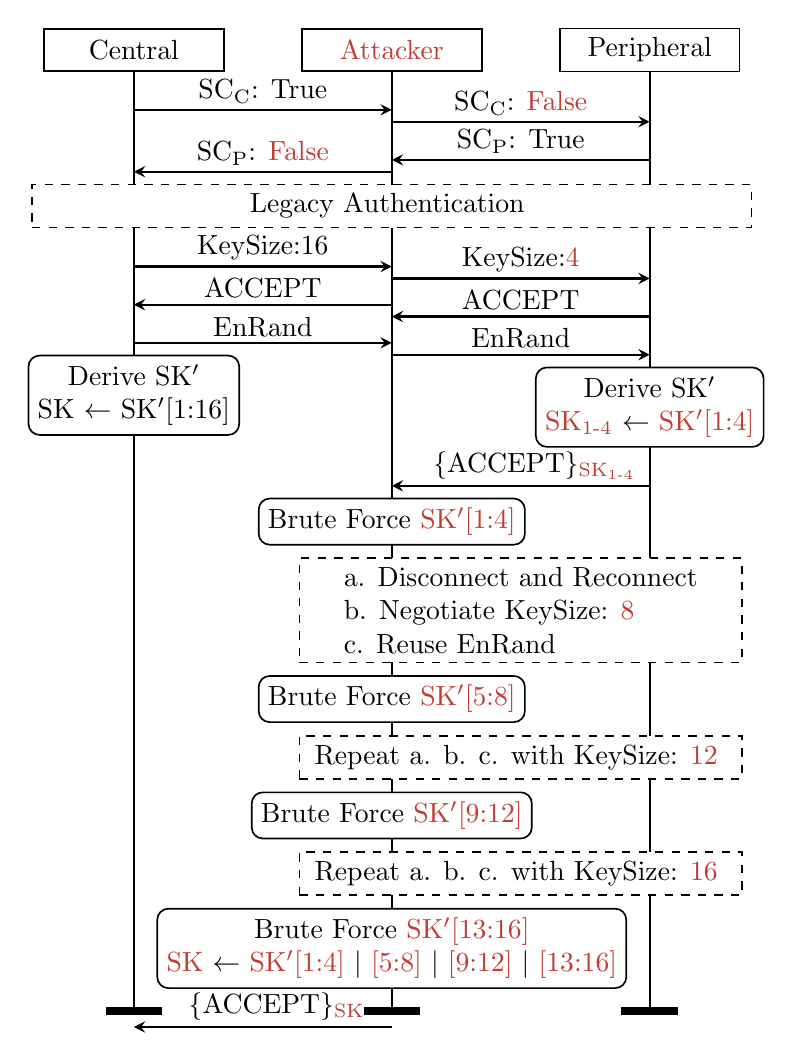
\begin{tikzpicture}

\node[AGENT] (n_initiator) {Central};
\node[AGENT, right=0.08\textwidth of n_initiator] (n_attacker) {\textcolor{xhs_red}{Attacker}};
\node[AGENT, right=0.08\textwidth of n_attacker] (n_responder) {Peripheral};

\coordinate (end_initiator) at ($(n_initiator.south)+(0,-78.5ex)$);
\draw[semithick] (n_initiator.south) -- (end_initiator);
\draw[fill=black] ($(end_initiator)+(-1em,0)$) rectangle ($(end_initiator)+(1em,-0.6ex)$);

\coordinate (end_attacker) at ($(end_initiator-|n_attacker)$);
\draw[semithick] (n_attacker.south) -- (end_attacker);
\draw[fill=black] ($(end_attacker)+(-1em,0)$) rectangle ($(end_attacker)+(1em,-0.6ex)$);

\coordinate (end_responder) at ($(end_initiator-|n_responder)$);
\draw[semithick] (n_responder.south) -- (end_responder);
\draw[fill=black] ($(end_responder)+(-1em,0)$) rectangle ($(end_responder)+(1em,-0.6ex)$);

\coordinate (c_init_sc) at ($(n_initiator.south)+(0,-3.2ex)$);
\coordinate (c_atta_sc) at ($(c_init_sc-|n_attacker)$);
\draw[ARROW] (c_init_sc) -- (c_atta_sc) node[midway,above=-0.3ex]{$\text{SC}_\text{C}$: True};

\coordinate (c_atta_sc) at ($(c_atta_sc)+(0,-1ex)$);
\coordinate (c_res_sc) at ($(c_atta_sc-|n_responder)$);
\draw[ARROW] (c_atta_sc) -- (c_res_sc) node[midway,above=-0.3ex]{$\text{SC}_\text{C}$: \textcolor{xhs_red}{False}};

\coordinate (c_res_sc) at ($(c_res_sc)+(0,-3.2ex)$);
\coordinate (c_atta_sc) at ($(c_res_sc-|n_attacker)$);
\draw[ARROW] (c_res_sc) -- (c_atta_sc) node[midway,above=-0.3ex]{$\text{SC}_\text{P}$: True};

\coordinate (c_atta_sc) at ($(c_atta_sc)+(0,-1ex)$);
\coordinate (c_init_sc) at ($(c_atta_sc-|n_initiator)$);
\draw[ARROW] (c_atta_sc) -- (c_init_sc) node[midway,above=-0.3ex]{$\text{SC}_\text{P}$: \textcolor{xhs_red}{False}};

\node[PREPARATION, minimum width=26em] (n_auth) at ($(c_atta_sc)+(0,-1ex)$) {
    Legacy Authentication
};

\coordinate (c_init_ks) at ($(n_auth.south-|n_initiator)+(0,-3.2ex)$);
\coordinate (c_atta_ksi) at ($(c_init_ks-|n_attacker)$);
\draw[ARROW] (c_init_ks) -- (c_atta_ksi) node[midway,above=-0.3ex]{KeySize:16};

\coordinate (c_atta_accept) at ($(c_atta_ksi)+(0,-3.2ex)$);
\coordinate (c_init_accept) at ($(c_atta_accept-|n_initiator)$);
\draw[ARROW] (c_atta_accept) -- (c_init_accept) node[midway,above=-0.3ex]{ACCEPT};

\coordinate (c_init_en) at ($(c_init_accept)+(0,-3.2ex)$);
\coordinate (c_atta_en) at ($(c_init_en-|n_attacker)$);
\draw[ARROW] (c_init_en) -- (c_atta_en) node[midway,above=-0.3ex]{EnRand};

\node[ACTION] (n_init_sk) at ($(c_init_en)+(0,-1ex)$) {Derive SK$'$\\SK $\leftarrow$ SK$'$[1:16]};

\coordinate (c_atta_ksr) at ($(c_atta_ksi)+(0,-1ex)$);
\coordinate (c_res_ksr) at ($(c_atta_ksr-|n_responder)$);
\draw[ARROW] (c_atta_ksr) -- (c_res_ksr) node[midway,above=-0.3ex]{KeySize:\textcolor{xhs_red}{4}};

\coordinate (c_res_accept) at ($(c_res_ksr)+(0,-3.2ex)$);
\coordinate (c_atta_accept) at ($(c_res_accept-|n_attacker)$);
\draw[ARROW] (c_res_accept) -- (c_atta_accept) node[midway,above=-0.3ex]{ACCEPT};

\coordinate (c_atta_en) at ($(c_atta_accept)+(0,-3.2ex)$);
\coordinate (c_res_en) at ($(c_atta_en-|n_responder)$);
\draw[ARROW] (c_atta_en) -- (c_res_en) node[midway,above=-0.3ex]{EnRand};

\node[ACTION] (n_res_sk) at ($(c_res_en)+(0,-1ex)$) {Derive SK$'$\\\textcolor{xhs_red}{$\text{SK}_\text{1-4}$} $\leftarrow$ \textcolor{xhs_red}{SK$'$[1:4]}};

\coordinate (c_res_encrypted) at ($(n_res_sk.south)+(0,-3.2ex)$); 
\coordinate (c_atta_encrypted) at ($(c_res_encrypted-|n_attacker)$);
\draw[ARROW] (c_res_encrypted) -- (c_atta_encrypted) node[midway,above=-0.3ex,xshift=0.5em]{$\{\text{ACCEPT}\}_{\textcolor{xhs_red}{\text{SK}_\text{1-4}}}$};

\node[ACTION] (n_atta_bf) at ($(c_atta_encrypted)+(0,-1ex)$) {Brute Force \textcolor{xhs_red}{SK$'$[1:4]}};

\coordinate (c_atta_res_middle) at ($(n_attacker)!0.5!(n_responder)$);

\node[PREPARATION, minimum width=16em,align=flush left] (n_atta_round1) at ($(n_atta_bf.south-|c_atta_res_middle)+(0,-1ex)$) {
    a. Disconnect and Reconnect\\
    b. Negotiate KeySize: \textcolor{xhs_red}{8} \\
    c. Reuse EnRand
};

% \node[ACTION] (n_res_round1) at ($(n_atta_round1.south-|n_responder)+(0,-1ex)$) {Derive SK$'$\\\textcolor{xhs_red}{$\text{SK}_\text{2}$} $\leftarrow$ \textcolor{xhs_red}{SK$'$[1:8]}};

% \coordinate (c_res_encrypted) at ($(n_res_round1.south)+(0,-1ex)$);
% \coordinate (c_atta_encrypted) at ($(c_res_encrypted-|n_attacker)$);
% \draw[ARROW] (c_res_encrypted) -- (c_atta_encrypted) node[midway,above=-0.3ex,xshift=-1em]{$\{\text{ACCEPT}\}_{\textcolor{xhs_red}{\text{SK}_2}}$};

\node[ACTION] (n_atta_bf) at ($(n_atta_round1.south-|n_attacker)+(0,-1ex)$) {Brute Force \textcolor{xhs_red}{SK$'$[5:8]}};

\node[PREPARATION, minimum width=16em,align=flush left] (n_atta_round2) at ($(n_atta_bf.south-|c_atta_res_middle)+(0,-1ex)$) {
    Repeat a. b. c. with KeySize: \textcolor{xhs_red}{12}
};

\node[ACTION] (n_atta_bf) at ($(n_atta_round2.south-|n_attacker)+(0,-1ex)$) {Brute Force \textcolor{xhs_red}{SK$'$[9:12]}};

\node[PREPARATION, minimum width=16em,align=flush left] (n_atta_round3) at ($(n_atta_bf.south-|c_atta_res_middle)+(0,-1ex)$) {
    Repeat a. b. c. with KeySize: \textcolor{xhs_red}{16}
};

\node[ACTION] (n_atta_bf) at ($(n_atta_round3.south-|n_attacker)+(0,-1ex)$) {
    Brute Force \textcolor{xhs_red}{SK$'$[13:16]}\\
    \textcolor{xhs_red}{SK} $\leftarrow$ \textcolor{xhs_red}{\text{SK$'$[1:4]}} $|$ \textcolor{xhs_red}{[5:8]} $|$ \textcolor{xhs_red}{[9:12]} $|$ \textcolor{xhs_red}{[13:16]}
    % \textcolor{xhs_red}{SK} $\leftarrow$ \textcolor{xhs_red}{\text{SK$'$[1:4]}} $|$ \textcolor{xhs_red}{\text{SK$'$[5:8]}} $|$ \textcolor{xhs_red}{\text{SK$'$[9:12]}}$|$ \textcolor{xhs_red}{\text{SK$'$[13:16]}}
};

\coordinate (c_atta_encrypted) at ($(n_atta_bf.south)+(0,-3.2ex)$);
\coordinate (c_init_encrypted) at ($(c_atta_encrypted-|n_initiator)$);
\draw[ARROW] (c_atta_encrypted) -- (c_init_encrypted) node[midway,above=-0.3ex,xshift=0.5em]{$\{\text{ACCEPT}\}_{\textcolor{xhs_red}{\text{SK}}}$};


\end{tikzpicture}

\end{document}
